\begin{figure}[!h]
  \centerline{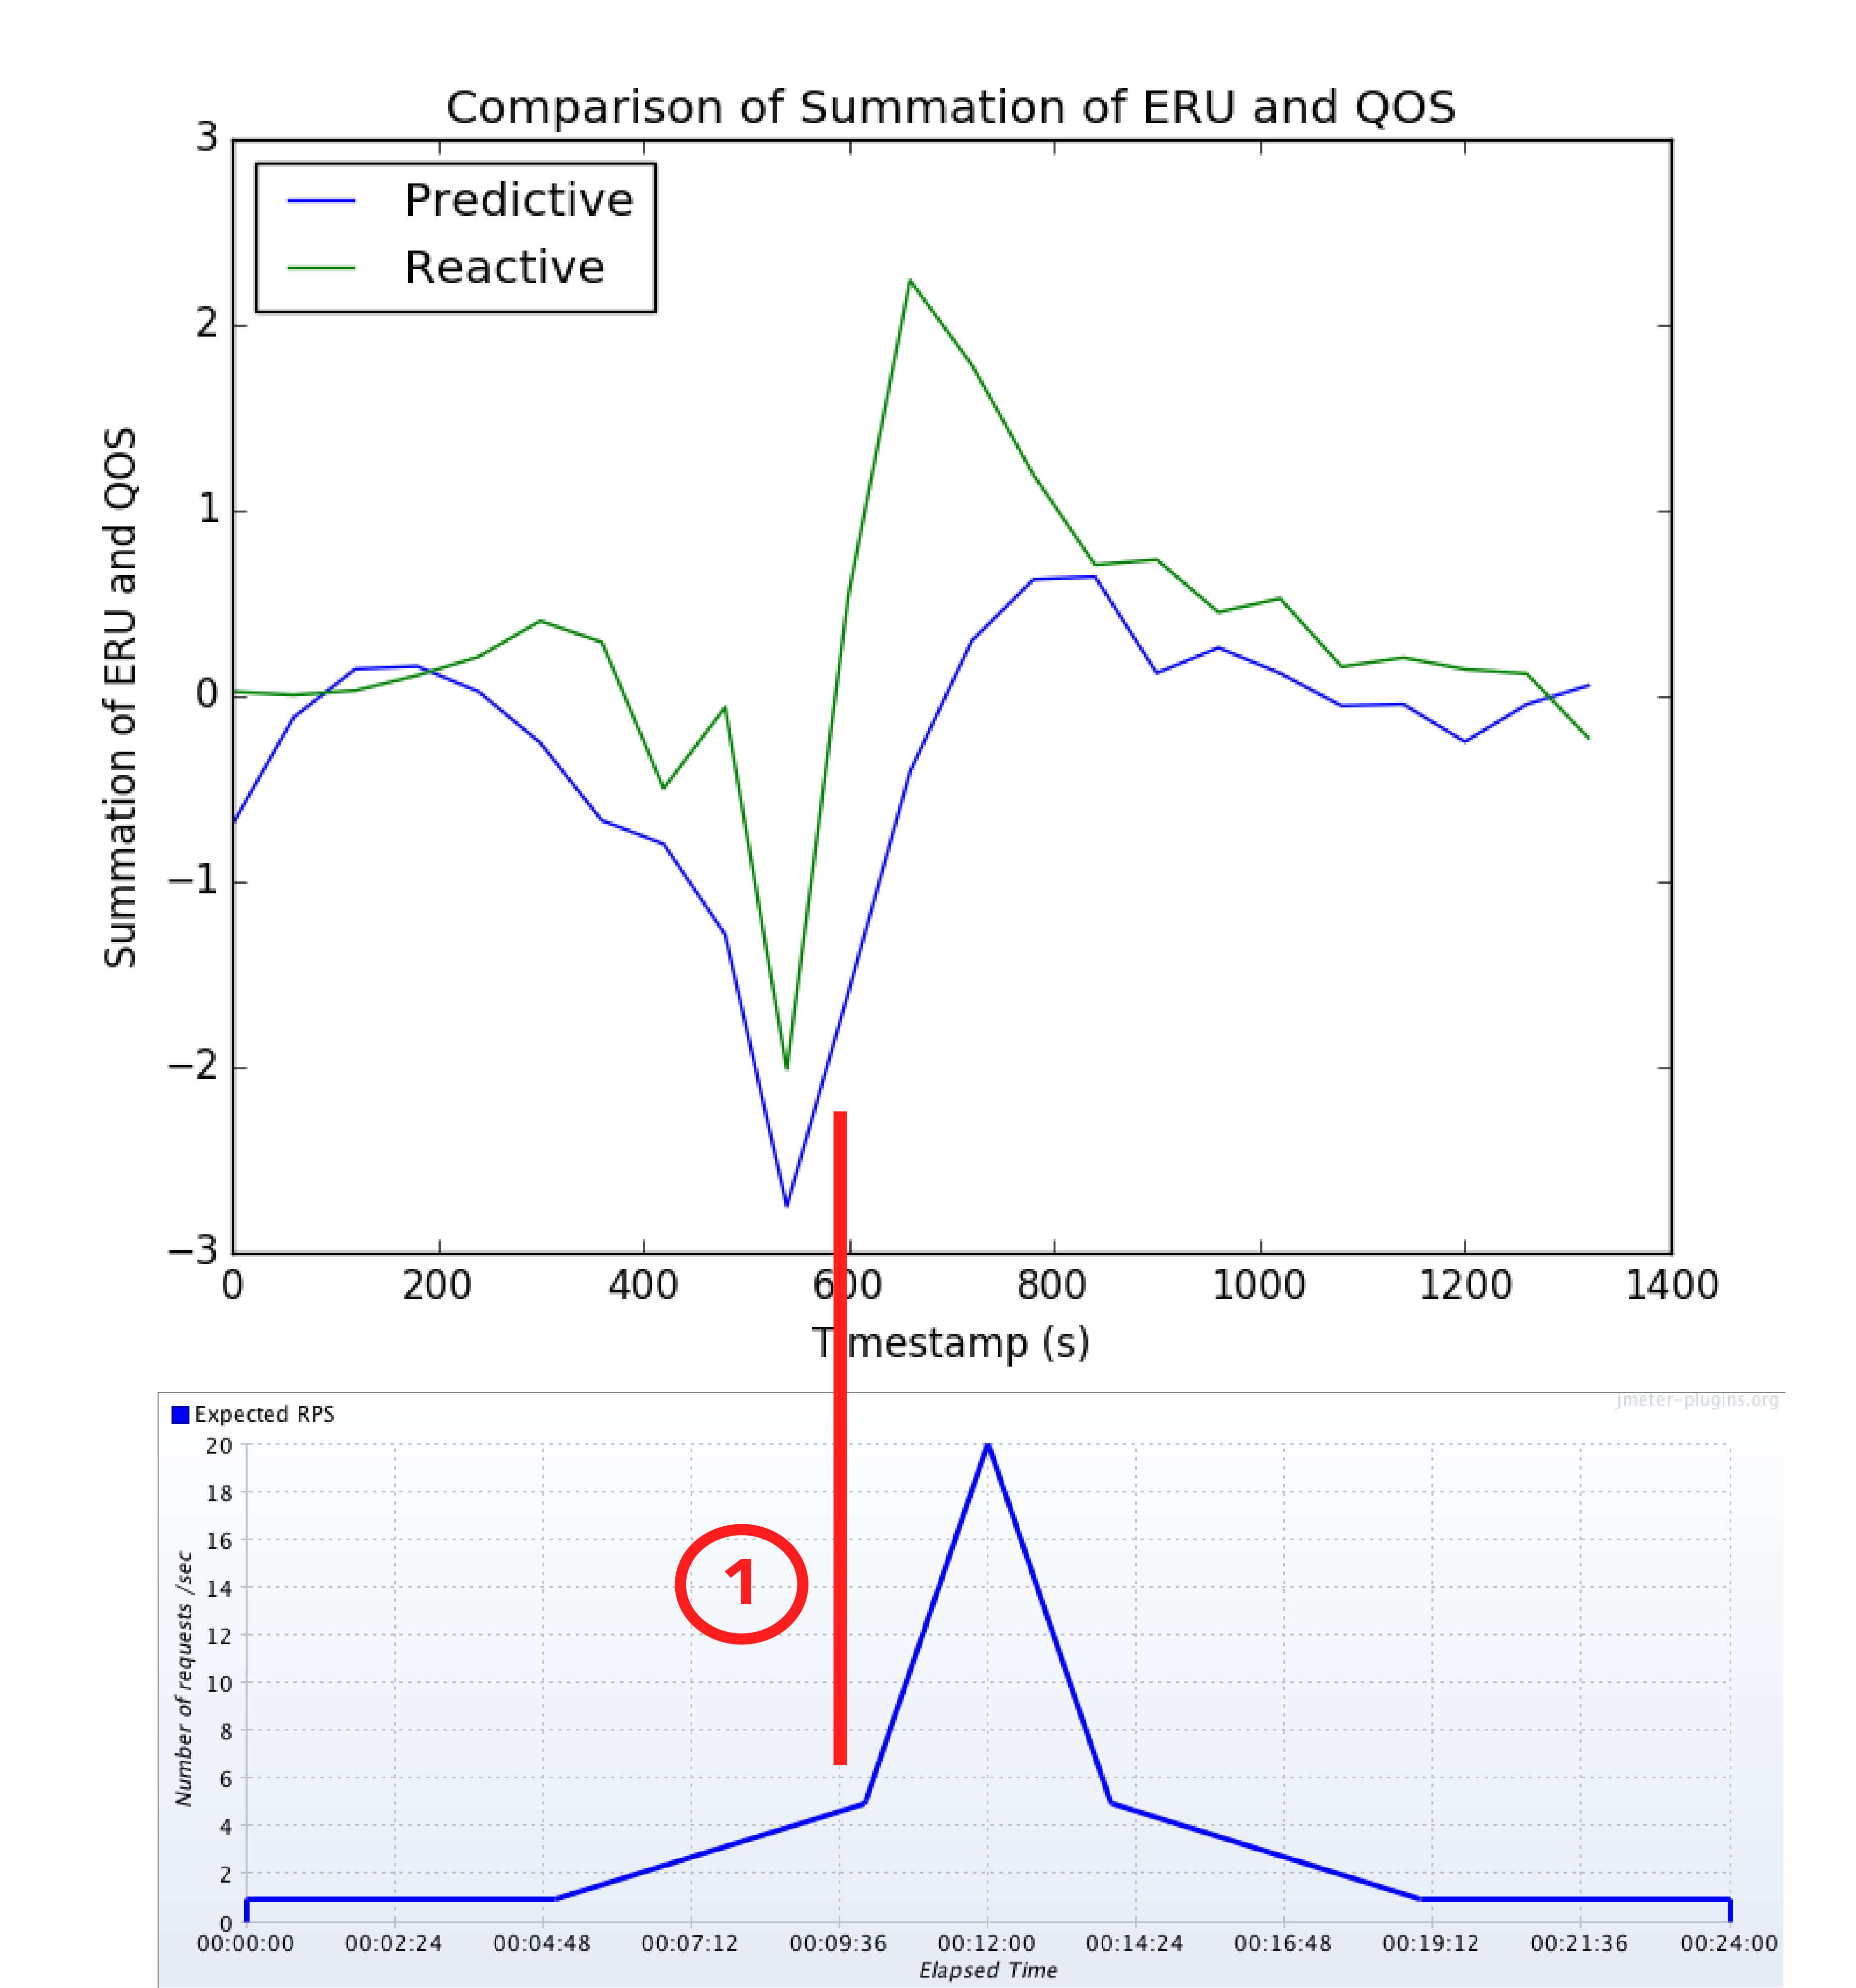
\includegraphics[scale=.70]{flash-crowd-short-labelled.png}}
  \caption{A comparison of the summation of ERU and QoS for
    predictive and reactive auto-scaling for 135s, flash-crowd.}
  \label{fig:135s-flash-crowd-labelled}
\end{figure}

Figure \ref{fig:135s-flash-crowd-labelled} contains a graph
showing predictive and reactive auto-scaling's different
summations of efficient resource utilization and quality of service over the
course of the \textit{flash-crowd} trial. Again,
we find that predictive auto-scaling is not particularly
beneficial in this context. Specifically, if we look at the moment labelled
$1$ on Figure \ref{fig:135s-flash-crowd-labelled}, we see another instance in which
predictive auto-scaling suffers a severe performance decrease because of
under-provisioning. Because this traffic pattern occurs over such a short
interval, the predictive auto-scaling algorithm is unable to fully recognize and
respond to the flash crowd, and is instead hampered by previous measurements
with a significantly lesser slope. Our line-of-best-fit for prediction has too
small a slope, and thus predictive auto-scaling functions worse than reactive
auto-scaling.

\begin{table}[htbp]
  \centering
  \caption{Difference in Predictive and Reactive Auto-scaling for 135s,
  flash-crowd.}
  \label{tab:135s-flash-crowd}
\begin{tabular}{l c}\hline\hline
    \multicolumn{1}{c}{\textbf{Measure}} & \textbf{Value} \\ \hline
     p-value & 0.802 \\
     z-score & -.850 \\
     std\_dev & 0.685 \\
     mean & -0.591
  \end{tabular}
\end{table}

Figure \ref{fig:135s-flash-crowd-labelled} shows that predictive
auto-scaling is fairly detrimental on the \textit{flash-crowd} traffic pattern.
Given Table \ref{tab:135s-flash-crowd}, we are still not able to claim
statistical significance with respect to these results, but we should be fairly
confident that this current iteration of predictive auto-scaling is not an advisable addition
when expecting flash crowds.
